\documentclass{beamer}

\usepackage{xltxtra}
\usepackage{xgreek}
\usepackage{url}
\usepackage{graphicx}
\usepackage{bbding}
\usepackage{gfsneohellenic}
\usetheme{Darmstadt}
\usecolortheme{crane}

\setsansfont[Mapping=tex-text]{GFS Neohellenic}

\title{Git}
\author{
Ομάδα Web}
\date{\today}

\begin{document}

\begin{frame}
\begin{minipage}{\hsize}
\centering
\end{minipage}
\titlepage
\end{frame}

\begin{frame}{Τι θα δούμε}
  \begin{itemize}
   \item Τι είναι ένα VCS (Version Control System);
   \pause
   \item Και τι να το κάνω εγώ αυτό;
   \pause
   \item Με λένε git!
   \pause
   \item Γιατί git;
   \pause
   \item Εντολές με PH>7.
   \pause
   \item Επιπλέον υλικό.
  \end{itemize}
\end{frame}

\begin{frame}{Τι είναι ένα Version Control System}
  \begin{itemize}
    \item Καταγράφει τις αλλαγές σε ένα σύνολο αρχείων
    \item Παρέχει δυνατότητα ανάκλησης προηγούμενων στιγμιοτύπων
    \item Διευκολύνει την διαχείριση κοινόχρηστων αρχείων
  \end{itemize}
\end{frame}

\begin{frame}{VCS.getCategories()}
  \begin{itemize}
    \item Local Version Control Systems
    \item Centralized Version Control Systems
    \begin{itemize}
      \item CVS, Subversion, Perforce
    \end{itemize}
    \item Distributed Version Control Systems
    \begin{itemize}
      \item \textbf{Git}, Mercurial, Bazaar, Darcs
    \end{itemize}
  \end{itemize}
\end{frame}

\begin{frame}{Και τι να το κάνω εγώ αυτό;}
 \begin{center}
    Σας θυμίζει κάτι αυτό;\\
    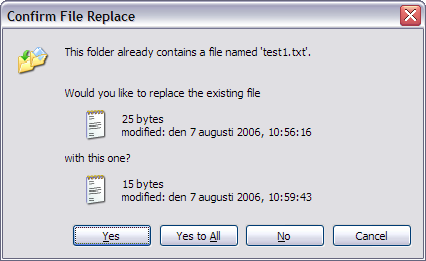
\includegraphics[scale=0.45]{replace.png}
  \end{center}
\end{frame}

\begin{frame}{Και τι να το κάνω εγώ αυτό;}
 Να το χρησιμοποιήσεις για τις ομαδικές εργασίες σου γιατί:
  \begin{itemize}
    \item Κρατάς - ελέγχεις εύκολα ιστορικό αλλαγών
    \pause
    \item Ανακαλείς τα αρχεία - project σε προηγούμενη κατάσταση
    \pause
    \item Παρέχει μια μορφή backup
    \pause
    \item Μπορείς να μοιραστείς εύκολα τον κώδικα
  \end{itemize}
\end{frame}

\begin{frame}{Με λένε git!}
 Αναπτύχθηκε από τον Linus Torvalds το 2005 για τη διαχείριση του κώδικα του Linux kernel
  \begin{itemize}
    \item Πλέον πολλές εταιρίες το χρησιμοποιούν για τη διαχείριση του κώδικα
    \pause
    \item Χρησιμοποιείται πολύ και από την open source κοινότητα
    \pause
    \item Διαθέσιμο παντού (όλα τα λειτουργικά, IDE extensions, terminal, μέσω GUI)
    \pause
    \item ΠΡΟΣΟΧΗ! Άλλο git και άλλο github!
  \end{itemize}
\end{frame}

\begin{frame}{Εντολές με PH>7}
\begin{itemize}
 \item git init
 \item git status
 \item git add -A
 \item git commit -m <message>
 \item git push
 \item git pull
 \item git clone
\end{itemize}
\end{frame}

\begin{frame}{Γενικό use case}
\begin{itemize}
  \item git clone <link to project>
  \item cd to project folder
  \item make changes
  \item git add -A
  \item git commit -m <message>
  \item git push origin master
\end{itemize}
\end{frame}

\begin{frame}{Επιπλέον υλικό}
\begin{columns}
  \column{.5\textwidth}
    \begin{figure}
      
\includegraphics[scale=0.1]{lifejacket.png}
    \end{figure}
  \column{.5\textwidth}
    \begin{block}{Links}
      \begin{itemize}
	\item  \href{http://git-scm.com/book}{Ανοικτό Βιβλίο}
	\item \href{http://try.github.io/levels/1/challenges/1}{Tutorial}
	\item \href{http://git-scm.com/book/ch4-2.html}{Στήσιμο git repo σε δικό μας server}
	\item \href{https://netbeans.org/kb/docs/ide/git.html}{Χρήση git με το Netbeans}
      \end{itemize}
    \end{block}
\end{columns}
\end{frame}

\begin{frame}{Για εσάς που είστε γάτες}
 \begin{center}
    Αφήστε το github και χρησιμοποιήστε το kithub! \\
    
\includegraphics[scale=0.45]{kithub.png}
  \end{center}
\end{frame}

\end{document}
